O programa MUSIC, a ser utilizado nas simulações deste trabalho, é um
gerador de eventos que pode ser encontrado em \cite{noauthor_music_nodate}.
\par
Em \cite{schenke_3+1d_2010} encontramos uma descrião mais detalhada do algoritmo empregado. Alguns fatos
são citados a seguir:

\begin{itemize}
 \item O método KURGANOV-TADMOR é implementado, este método baseia-se na introdução de
 um termo de dissipação numérica para garantia de estabilidade, é capaz de lidar com
 choques e descontinuidades, ideal para a inserção de termos fonte como deposição de energia
 de jatos;
 \item As condições iniciais são baseadas no modelo de Glauber e na parametrização de Woods-Saxon,
 ver subseção \ref{glauber};
 \item Uma simplificação das equações é atingida escolhendo variáveis através de uma rotação hiperbólica;
 \item O {\it freeze-out} é construído assumindo a fórmula de Cooper-Frye\cite{teaney_chemical_2002};
\end{itemize}

É interessante observar na Figura \ref{fig:musicv2} que o MUSIC não fornece resultados coerentes com os experimentos na faixa de $p_T$
entre $1$ e $2 GeV$. Isso poderia ser explicado pela ausência de energia depositada pelos jatos, que incluem na hidrodinâmica efeitos
anisotrópicos\cite{andrade_jet_2014}, ver Figura \ref{fig:v2}.

\begin{figure}[!h]
\centering
 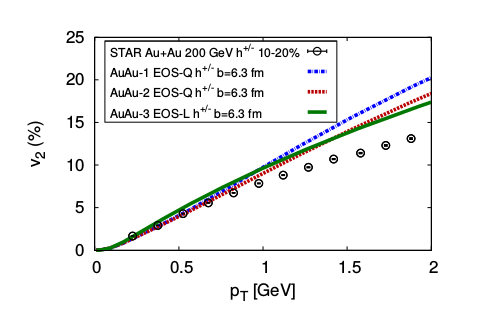
\includegraphics[scale=0.5]{Content/music_results.png}
 \caption{Resultados do MUSIC no coeficiente $V_{2}$.}
 \label{fig:musicv2}
\end{figure}
